\documentclass{article}
\usepackage{graphicx} % Required for inserting images
\usepackage{tcolorbox} % Required for the colored box
\usepackage{caption}
\usepackage{verbatim}


% Define a custom command for section headings
\newcommand{\heading}[1]{\noindent\textcolor{gu-green}{\textbf{\large #1}}}

\begin{document}

\begin{titlepage}
  \begin{center}
  
    
    % Insert the university logo
    
\includegraphics[width=0.4\textwidth]{logo.svg.png}
    
    {\LARGE\textbf{Green University of Bangladesh}}\\
    \vspace{0.5cm}
    {\Large Department of Computer Science and Engineering}\\
    \vspace{1cm}
    
    \rule{\linewidth}{0.5mm}
    
    \vspace{0.5cm}
    {\LARGE\textbf{Lab Report}}\\
    \vspace{0.5cm}
    {\Large Course Title: Object Oriented Programming Lab}\\
    \vspace{0.2cm}
    {\Large Course Code: CSE-221 Section: DA}\\
    \vspace{0.5cm}
   \rule{\linewidth}{0.5mm}
    \vspace{1cm}
    \LARGE \textbf{} Experiment Title : \LARGE Java Syntax Similarity: Array, Conditionals, Loops\\
     \LARGE \textbf{} Lab Report No: \LARGE 01\\
     \LARGE \textbf{} Semester: \LARGE Spring, Year: 2023\\
    \vspace{0.5cm}
    \LARGE \textbf{} Program: B.Sc in CSE (Day)\\
    
    \vspace{3cm}
    \begin{tcolorbox}[colback=white,colframe=black,width=10cm,height=2cm]
      \LARGE{Student Name:} IBRAHIM REFAT \\
      \textbf{ID:} 221902333 \\
    \end{tcolorbox}
    
    \vspace{2cm}
    \textbf{Lab Date:} 20/02/2023 \\
    \vspace{0.2cm}
  \textbf{Submission Date:} 26/02/2023 \\
    \vspace{0.2cm}
   \textbf{Course Teacher:} Dr. Muhammad Aminur Rahaman
    
  \end{center}
\end{titlepage}

% Start the main content on a new page
\clearpage

\section{Title}
\Large 01. Implement checking of odd and even number \newline
\Large 02. Implement summation of factorial odd number series.
\section{Objective}
\large 1. Through the first problem, we will learn how to determine whether a number is even or odd and how to take input from the user. This section will also introduce us to the use of loops.

\large 2. In the second problem, we will explore the sum of factorial odd number series. This problem will provide us with the opportunity to learn how to apply loops and conditionals.

\section{Procedure}
\Large Problem : 01
\begin{enumerate}
\item Start
\item  Declare an integer variable "number"
\item  Read a number from the user and store it in "number"
\item  Calculate the remainder of "number" divided by 2 using the modulo operator (%)
\item  If the remainder is equal to 0, print "number is even"
\item  If the remainder is not equal to 0, print "number is odd"
\item  Exit

\end{enumerate}
\vspace{0.5cm}
\Large Problem : 02
\begin{enumerate}
    \item Start
    \item Take two input from user value and a power value
    \item Read and store enterd value
    \item Check the entered power value.
    \item if power is even then continue else break
    \item every power have to even for that we start loop from 2 and i+=2.
    \item Now, we calculate summation of factorial odd serise  $x^n / (n-1)!$
    \item End
\end{enumerate}



\begin{enumerate}
    \item 
    
\end{enumerate}


\section{Implementation}
{\Large \textbf{Problem : 01}}
\begin{verbatim}
package com.problemsolve.evenoddnubercheck;

/**   
 *   
 * @author ibrahim refat    
 */   
import java.util.Scanner;  
public class EvenOddNuberCheck {

    public static void main(String[] args) {
         
        Scanner scan = new Scanner(System.in);
        int number;
        System.out.print("Enter a number : ");
         number = scan.nextInt();
         if(number % 2 ==0)
         {
             System.out.println(number +" is a Even number");
         }
         else System.out.println(number+" is Odd number");
    }
}
\end{verbatim}

\vspace{0.5cm}

{\Large \textbf{Problem : 02}}

\begin{verbatim}
package com.problemsolve.summationoffactorialoddnumber;

/**
 *
 * @author ibrahim rifat
 */
import java.util.Scanner;

public class SummationOfFactorialOddNumber {

    public static void main(String[] args) {
         
        Scanner scan = new Scanner(System.in);
        System.out.print("Enter base : ");
        double base = scan.nextDouble();
        System.out.print("Enter power : ");
        int power = scan.nextInt();
        
        if(power % 2==0){
            double sum = 0 ;
            
     for(int i = 2; i <= power; i+= 2){
     double cal = Math.pow(base,i) / factorial(i - 1);
    sum += cal;
     }
System.out.println("Sum of factorial odd number serise : "+sum);
        }
        
     else {
System.out.println(" Your given number is wrong");
        }
    
            
    }
    
    public static double factorial(int n) {
        double result = 1;
        for (int i = 2; i <= n; i++) {
            result *= i;
        }
        return result;
    }
    
}
 

\end{verbatim}



\section{Test Result}
\large \textbf{01}
 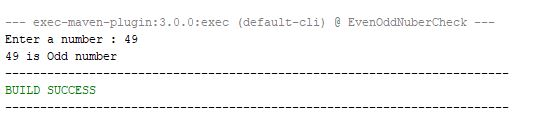
\includegraphics[width=1\textwidth]{problem1.JPG}
 \centering
\large Figure 01 : Even / Odd number check
\vspace{0.5cm}

\large \textbf{02}
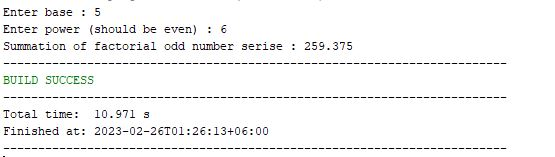
\includegraphics[width=1\textwidth]{problem2.JPG}
 \centering
 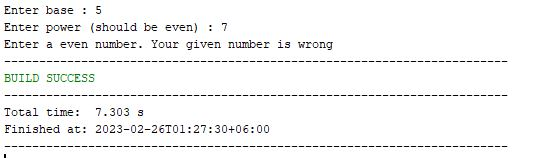
\includegraphics[width=1\textwidth]{problem3.JPG}
 \centering
\large Figure 02 : Summation of factorial odd serise

 
\section{ANALYSIS AND DISCUSSION}
 I had to face many problems while solving the second problem because the task was to find the sum of factorials of odd numbers. I solved the problem by checking the validity of the input using conditional statements and by taking only even numbers in the for loop. I outputted the value of the factorial using a method. While solving the second problem, I encountered many errors but I learned to handle unexpected errors effectively.

  

 

\end{document}
